\chapter{METODOLOGI}

\section{Alat dan Bahan}
Bahan yang digunakan dalam penelitian ini adalah:

\vspace{-0.5cm}

\begin{enumerate}[a.]
\begin{singlespace}
\itemsep0em
\item Kit pancar-rima (10 unit),
\item Kit pengembangan program (2 unit),
\item Kit pengunduh program (2 unit),
\item Asesoris kit pancar-rima (10 unit),
\item Kit ekspansi (5 unit),
\item Access Point (3 unit).
\end{singlespace}
\end{enumerate}

\section{Langkah Kerja}
Rancangan arsitektur yang akan digunakan pada penelitian ini diilustrasikan seperti pada Gambar \ref{wifi}. Pada gambar tersebut diilustrasikan sebuah sistem yang terdiri atas dua buah WSN dengan protokol yang berbeda dan satu buah jaringan nirkabel lokal (WiFi). Protokol WSN yang akan digunakan dalam penelitian ini adalah dari IQRF dan ZigBee. Pelaksanaan penelitian ini akan dibagi menjadi tiga paket pekerjaan (Work Package, WP).

\textbf{WP 1: Perancangan Perangkat Lunak}

Pada tahap ini akan dilakukan studi literatur yang dititikberatkan pada sistem operasi (Operating System, OS) untuk piranti tertanam (embedded device). Langkah selanjutnya adalah rerancangan perangkat lunak yang akan ditanamkan pada Access Point (AP). Perangkat lunak yang akan ditanamkan harus bekerja secara efisien karena kemampuan komputasi yang terbatas pada AP.

\begin{figure}[ht!]
  \centering
    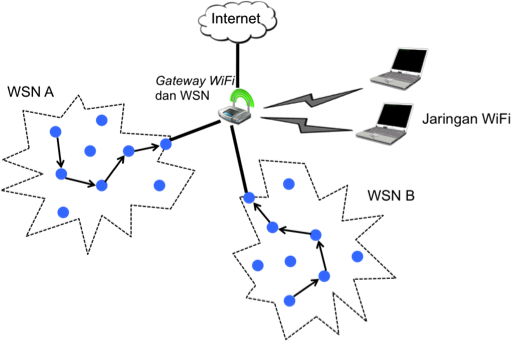
\includegraphics{gambar/wifi}
    \caption{Arsitektur WSN dan WiFi dengan sebuah AP.}
    \label{wifi}
\end{figure}

\textbf{WP 2: Implementasi Perangkat Lunak}

Implementasi perangkat lunak dilakukan pada tahap ini. Langkah pertama yang dilakukan adalah memastikan bahwa WSN dapat terhubungan dengan internet sesuai dengan yang direncanakan. Langkah selanjutnya adalah memastikan bahwa jaringan WiFi tidak mengalami gangguan setelah perangkat lunak yang baru tertanam pada AP. Penambahan layanan-layanan yang diperlukan dapat pula dilakukan pada tahap ini.

\textbf{WP 3: Integrasi dan Pengujian Seluruh Sistem}

Jika jaringan WiFi dan dua protokol WSN masing-masing dapat berhubungan dengan internet, maka pada tahap ini akan dilakukan pengujian sistem secara keseluruhan. Pengujian dinaikkan dari skala lab menjadi skala \emph{test-bed}. Pengujian dalam \emph{test-bed} dilakukan untuk menjamin bahwa sistem yang dikembangkan bekerja sesuai dengan yang direncanakan.

\section{Jadwal Kegiatan}
Penelitian direncanakan akan dilaksanakan selama enam bulan. Rincian rencana jadwal penelitian dicantumkan dalam tabel berikut.

\begin{center}
Tabel 3.1. Jadwal Penelitian.
\end{center}
\vspace{-0.5cm}
\begin{figure}[ht!]
  \centering
    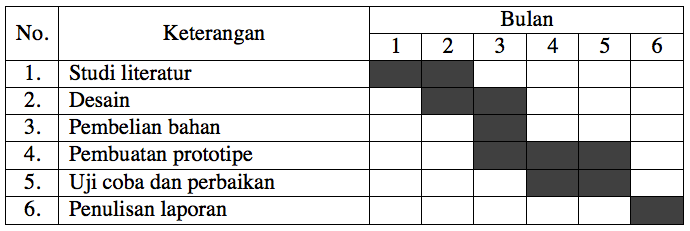
\includegraphics[width=13cm]{gambar/timeline}
\end{figure}